% ============================================================
% articulo.tex — Borrador del artículo técnico (formato IEEE, CATT ESCOM-IPN)
% Trabajo Terminal 2026-B039
% Síntesis de Docs/capitulos/0_Preliminares/resumen.tex, 1_Panorama_General/,
% 5_Metodologia/, 6_Resultados/ y 7_Conclusiones/.
% Entradas que lo respaldan: D-008, D-009, D-010, D-012, D-013, D-014, D-016,
% D-017, D-019, D-020, D-021, D-023, D-024, D-025, D-026, D-027, D-028, D-029,
% D-031, D-032, D-033, D-035, D-036, D-038, D-039, D-040, D-042, H-002, H-005,
% H-012, H-013, H-018, H-019, H-020, H-021, H-023, H-024, H-025, H-026, H-027,
% H-028, H-031, H-032, H-034, H-035, H-036, H-037, H-038, H-039, H-040, H-041,
% H-042, H-043, H-044, H-045, H-046, H-047, H-048, H-049, H-050, H-051, H-052,
% H-053, H-054, H-055.
% ============================================================
\documentclass[conference,letterpaper]{IEEEtran}

\usepackage[utf8]{inputenc}
\usepackage[T1]{fontenc}
\usepackage[spanish,es-tabla,es-nodecimaldot,es-noshorthands]{babel}
\usepackage{amsmath}
\usepackage{amssymb}
\usepackage{graphicx}
\usepackage{booktabs}
\usepackage{array}
\usepackage{url}

\graphicspath{{../Figures/}}

\addto\captionsspanish{%
  \renewcommand{\abstractname}{Resumen}%
  \renewcommand{\IEEEkeywordsname}{Palabras clave}%
  \renewcommand{\refname}{Referencias}%
  \renewcommand{\tablename}{TABLA}%
  \renewcommand{\figurename}{Fig.}%
}
\renewcommand{\IEEEkeywordsname}{Palabras clave}

\setlength{\emergencystretch}{2em}

\title{Modelo de transformación cuántica variacional de características de cáncer de mama para un sistema híbrido de prediagnóstico}

\author{\IEEEauthorblockN{Miguel Alexander Sánchez García, Jesús Yaljá Montiel Pérez, Ana María Winfield Reyes}
\IEEEauthorblockA{Escuela Superior de Cómputo, Instituto Politécnico Nacional, Ciudad de México\\
Tel. 57-29-6000 ext. 52000 y 52021. E-mail: msanchezg1904@alumno.ipn.mx}%
% [VERIFICAR: correo de los directores]
}

\begin{document}

\maketitle

\begin{abstract}
% fuente: Docs/capitulos/5_Metodologia/5.3_M1_lectura.tex:62, Docs/capitulos/5_Metodologia/5.5_M3_extraccion.tex:10, Docs/capitulos/5_Metodologia/5.6_M4_seleccion.tex:11, Docs/capitulos/5_Metodologia/5.6_M4_seleccion.tex:41, Docs/capitulos/6_Resultados/6.2_separabilidad.tex:12, Docs/capitulos/6_Resultados/6.2_separabilidad.tex:17, Docs/capitulos/6_Resultados/6.2_separabilidad.tex:77, Docs/capitulos/6_Resultados/6.2_separabilidad.tex:78, Docs/capitulos/6_Resultados/6.8_sintesis.tex:35, Docs/capitulos/6_Resultados/6.4_qsvm_ventaja.tex:13, Docs/capitulos/6_Resultados/6.6_restricciones_simulador.tex:26 (H-031, H-038, H-039, H-042, H-044, H-051, H-052; 5b_concentracion_kernel.csv, 6_alineamiento_kernel.csv, 6_diferencia_geometrica_resumen.csv, 7_test.csv, X4_test_diferencias.csv, 8_oe6_shots_kernel.csv)
En este artículo se evalúa la viabilidad de las transformaciones cuánticas variacionales como mecanismo de codificación de características radiómicas de mamografías reales. Sobre las 3\,568 lesiones del conjunto de datos CBIS-DDSM, procesando masas y calcificaciones como subproblemas independientes, se extraen 67 características radiómicas mediante PyRadiomics, se seleccionan 12 con filtro de colinealidad y se escalan al intervalo $[0,\pi]$ por cuantiles. El mismo vector alimenta cinco condiciones experimentales: sin transformación (C1), análisis de componentes principales lineal como control nulo (C2), Kernel PCA con kernel gaussiano RBF (C3) y dos mapas de características cuánticos en Qiskit Aer (\texttt{zz\_\allowbreak feature\_\allowbreak map} en C4 y \texttt{pauli\_\allowbreak feature\_\allowbreak map} con términos $Y$ y $ZZ$ en C5) acoplados a un circuito variacional de parámetros fijos. La separabilidad se cuantifica mediante alineamiento kernel-objetivo (KTA), diferencia geométrica regularizada $g$, dimensión efectiva, índice de Davies-Bouldin y razón de Fisher; la clasificación se evalúa con un mismo perceptrón multicapa (MLP) bajo validación cruzada agrupada por paciente. Las representaciones cuánticas no muestran mayor separabilidad en ninguna métrica: a escala nominal ($c = 1$), el kernel cuántico se encuentra concentrado (mediana fuera de la diagonal de 0.0022 a 0.0029 en C4 y de 0.000031 a 0.000032 en C5, frente a 0.607 del RBF) y la diferencia geométrica mínima ($g$ de 1.400 a 1.701) permanece muy por debajo del umbral $\sqrt{N} \approx 14.1$. En el conjunto de prueba, el MLP registra entre 0.07 y 0.14 menos de AUC-ROC sobre los \textit{embeddings} cuánticos, mientras que un clasificador de vectores de soporte sobre el kernel cuántico de C4 supera al MLP en $+0.10$ a $+0.13$ de AUC-ROC e iguala al SVM clásico, ubicando la pérdida en la reducción del estado cuántico a 12 valores esperados locales $\langle Z_i \rangle$. Asimismo, se documentan las restricciones operacionales del simulador y de la medición física: con 1\,024 disparos, entre el 15.7\,\% y el 74.5\,\% de las entradas fuera de la diagonal del kernel cuántico se leerían exactamente como cero.
\end{abstract}

\begin{IEEEkeywords}
aprendizaje automático cuántico, \textit{quantum embeddings}, kernels cuánticos, separabilidad de clases, radiómica, CBIS-DDSM, cáncer de mama.
\end{IEEEkeywords}

\section{Introducción}

El cáncer de mama es la neoplasia diagnosticada con mayor frecuencia en mujeres a nivel mundial y constituye la primera causa de muerte por tumores malignos en mujeres tanto en el mundo como en México \cite{Bray2024GLOBOCAN, INEGI2025}. Aunque el tamizaje mamográfico oportuno reduce sustancialmente la mortalidad, la interpretación visual presenta variabilidad entre observadores y enfrenta limitaciones ante tejido mamario denso y cargas crecientes de lectura en los sistemas de salud. Estas restricciones han impulsado el desarrollo de sistemas de diagnóstico asistido por computadora (CADx); no obstante, los modelos basados en aprendizaje profundo suelen exhibir caídas pronunciadas de desempeño al evaluarse en distribuciones externas a las de su entrenamiento \cite{Wang2020DeepLearning}, además de operar sobre representaciones internas sin interpretación morfológica directa. En contraste, el enfoque radiómico extrae descriptores explícitos de intensidad, forma y textura de la región de interés (ROI), permitiendo auditar qué propiedades físicas conserva o altera cada transformación del flujo de procesamiento.

% fuente: Docs/capitulos/5_Metodologia/5.7_M5_transformacion.tex:115, Docs/capitulos/6_Resultados/6.2_separabilidad.tex:78 (D-027, H-038, H-039)
En el aprendizaje automático cuántico, un circuito de codificación $U(\mathbf{x})$ define una transformación no lineal $\phi: \mathbb{R}^k \to \mathcal{H}$ que asocia cada vector clásico $\mathbf{x}$ con un estado cuántico $|\phi(\mathbf{x})\rangle$ en un espacio de Hilbert de dimensión $2^k$, cuya geometría de similitud queda determinada por el kernel de fidelidad $K_Q(\mathbf{x},\mathbf{x}') = |\langle\phi(\mathbf{x})|\phi(\mathbf{x}')\rangle|^2$ \cite{havlicek2019supervised, schuld2019quantum}. Integrados con capas clásicas, estos circuitos conforman arquitecturas híbridas en las que el bloque cuántico actúa como una transformación entre espacios vectoriales \cite{Mari2020Transfer}. Sin embargo, estudios comparativos recientes muestran que los clasificadores clásicos estándar suelen igualar o superar a los modelos cuánticos de pequeña escala y que suprimir el entrelazamiento a menudo no degrada el rendimiento \cite{Bowles2024Benchmarking}. Desde el punto de vista teórico, Huang et al.~\cite{huang2021power} demostraron que cuando la diferencia geométrica $g$ entre el kernel cuántico y los kernels clásicos es pequeña ($g \ll \sqrt{N}$), un modelo clásico garantiza un desempeño predictivo similar o superior para cualquier etiquetado, fenómeno frecuente cuando el crecimiento exponencial del espacio de Hilbert coloca las muestras casi ortogonales entre sí. De forma complementaria, Thanasilp et al.~\cite{Thanasilp2024} probaron que la expresividad del mapa y el entrelazamiento pueden inducir una concentración exponencial de las fidelidades hacia un valor fijo, haciendo que la estimación con un número polinomial de disparos (\textit{shots}) produzca modelos insensibles a las entradas.

% fuente: Docs/capitulos/5_Metodologia/5.3_M1_lectura.tex:62, Docs/capitulos/5_Metodologia/5.6_M4_seleccion.tex:11 (D-012, D-013, D-019)
En mamografía, el antecedente directo es el estudio de Azevedo et al.~\cite{Azevedo2022QuantumTransfer}, quienes, entre otras líneas de trabajo futuro, propusieron procesar masas y calcificaciones por separado antes de clasificar y analizar cómo se distribuyen las lesiones dentro del espacio de Hilbert. El presente trabajo retoma esas dos líneas sobre las 3\,568 lesiones del conjunto de datos público CBIS-DDSM \cite{Lee2017CBISDDSM}, evaluando si las transformaciones cuánticas implementadas con \texttt{zz\_\allowbreak feature\_\allowbreak map} y \texttt{pauli\_\allowbreak feature\_\allowbreak map} en $k = 12$ qubits modifican la separabilidad entre lesiones benignas y malignas respecto a representaciones clásicas construidas desde el mismo vector radiómico, en qué medida dichas diferencias se trasladan a un mismo clasificador neuronal y cuáles son las restricciones prácticas del simulador y de la medición cuántica.

\section{Metodología}

El sistema se estructura en ocho módulos secuenciales (M1 a M8). En todo el flujo, los subconjuntos de masas y de calcificaciones se procesan como subproblemas independientes, dado que difieren en su presentación radiológica y en la distribución de sus descriptores.

\subsection{Lectura, preprocesamiento y extracción (M1--M3)}

% fuente: Docs/capitulos/5_Metodologia/5.3_M1_lectura.tex:29, Docs/capitulos/5_Metodologia/5.3_M1_lectura.tex:59, Docs/capitulos/5_Metodologia/5.3_M1_lectura.tex:62, Docs/capitulos/6_Resultados/6.1_datos_caracteristicas.tex:23, Docs/capitulos/6_Resultados/6.1_datos_caracteristicas.tex:33, Docs/capitulos/6_Resultados/6.2_separabilidad.tex:20, Docs/capitulos/6_Resultados/6.6_restricciones_simulador.tex:13 (D-012, H-002, H-020, H-021, H-023)
El Módulo~1 unifica los cuatro archivos de metadatos del CBIS-DDSM \cite{Lee2017CBISDDSM} y resuelve las rutas hacia los archivos DICOM de 16 bits en convención \texttt{MONOCHROME2}. Tras recuperar 84 series faltantes mediante la interfaz de programación de TCIA (pasando del 97.6\,\% al 100\,\% de cobertura), se integraron los 3\,568 registros completos distribuidos en 3\,103 mamografías: 1\,696 lesiones de masas (1\,318 en entrenamiento, con 637 malignas y 681 benignas) y 1\,872 de calcificaciones (1\,546 en entrenamiento, con 544 malignas y 1\,002 benignas), sumando 2\,864 lesiones de entrenamiento. La etiqueta patológica se codifica de forma binaria ($0 = \text{benigno}$, incluyendo \texttt{BENIGN\_\allowbreak WITHOUT\_\allowbreak CALLBACK}; $1 = \text{maligno}$). Ninguno de los archivos DICOM contiene el atributo \texttt{PixelSpacing} ni \texttt{Manufacturer}, por lo que los descriptores geométricos quedan expresados en píxeles.

% fuente: Docs/capitulos/5_Metodologia/5.4_M2_preprocesamiento.tex:13, Docs/capitulos/5_Metodologia/5.4_M2_preprocesamiento.tex:20, Docs/capitulos/5_Metodologia/5.4_M2_preprocesamiento.tex:25, Docs/capitulos/5_Metodologia/5.4_M2_preprocesamiento.tex:30, Docs/capitulos/6_Resultados/6.1_datos_caracteristicas.tex:16 (D-009, D-010, D-020, D-021, H-020; 2_preprocesamiento_qa.csv)
El Módulo~2 alinea cada mamografía completa con su máscara ROI binaria. En 80 de los 3\,568 registros las dimensiones diferían entre imagen y máscara: 78 masas cuyas máscaras estaban escaladas por un factor de 0.870 en ambos ejes se remuestrearon mediante vecino más cercano, y 2 calcificaciones con desplazamiento de pocas decenas de píxeles se anclaron sin escalar. La alineación se verificó frente a los recortes de referencia en 3\,206 de 3\,213 casos evaluables (99.8\,\%); los 7 casos discordantes en masas se conservaron y declararon, pues excluirlos del conjunto de prueba altera el AUC en menos de 0.004. Posteriormente, cada máscara se redujo a su componente conexa mayor (el 86.3\,\% de las máscaras de masas presentaba islas periféricas de pocos píxeles, reteniendo la componente principal al menos el 99.55\,\% del área) y se extrajo el recorte de la caja mínima ampliada en 20 píxeles por lado, manteniendo la resolución espacial original y las intensidades crudas de 16 bits. No se emplearon los recortes pregenerados del CBIS-DDSM debido a que presentan ganancias de intensidad variables entre 1.00 y 5.31, ni se redimensionó a una malla fija de $224\times 224$ para no destruir las variables morfológicas de tamaño. Conforme a las directrices de estandarización de la iniciativa IBSI \cite{Zwanenburg2020IBSI}, la ecualización local CLAHE se excluyó de la ruta principal y se reservó para una comparación de sensibilidad sobre imágenes convertidas a 8 bits.

% fuente: Docs/capitulos/5_Metodologia/5.5_M3_extraccion.tex:10, Docs/capitulos/5_Metodologia/5.5_M3_extraccion.tex:14, Docs/capitulos/5_Metodologia/5.5_M3_extraccion.tex:26 (D-008, D-023)
En el Módulo~3 se extrajeron 67 características radiómicas por lesión mediante PyRadiomics \cite{vanGriethuysen2017} sobre la imagen original sin filtros: 18 de intensidad de primer orden, 9 de forma bidimensional, 24 de matriz de coocurrencia de niveles de gris (GLCM) y 16 de matriz de longitud de rachas (GLRLM), promediando las cuatro direcciones del plano a distancia 1. La discretización de intensidades se fijó en un número constante de 32 niveles (\texttt{binCount}), siguiendo la recomendación de IBSI para unidades de intensidad arbitrarias no calibradas \cite{Zwanenburg2020IBSI}.

\subsection{Selección, escalado y transformación cuántica (M4--M5)}

% fuente: Docs/capitulos/5_Metodologia/5.6_M4_seleccion.tex:11, Docs/capitulos/5_Metodologia/5.6_M4_seleccion.tex:17, Docs/capitulos/5_Metodologia/5.6_M4_seleccion.tex:30, Docs/capitulos/5_Metodologia/5.6_M4_seleccion.tex:38, Docs/capitulos/5_Metodologia/5.6_M4_seleccion.tex:53, Docs/capitulos/6_Resultados/6.1_datos_caracteristicas.tex:103, Docs/capitulos/6_Resultados/6.1_datos_caracteristicas.tex:111 (D-013, D-024, D-025, D-026, H-026, H-027, H-028; 4_seleccion.csv, 4_semilla_folds.csv)
El Módulo~4 reduce el vector radiómico a $k = 12$ dimensiones y lo escala al dominio angular $[0,\pi]$, ajustando todos los parámetros exclusivamente sobre el conjunto de entrenamiento. El valor $k = 12$ se estableció mediante un estudio previo de escalabilidad (donde evaluar los kernels por circuitos individuales pasaba de 2.95~h con 12 qubits a 41.25~h con 16 qubits) y para dar cabida a múltiples familias radiómicas. Las variables se ordenan de forma decreciente según el estadístico $F$ de ANOVA univariante y se incorporan secuencialmente solo si su correlación lineal absoluta de Pearson con las ya aceptadas satisface $|r| \le 0.95$, evitando duplicados analíticos \cite{Guyon2003}. Cada variable seleccionada $r_i$ se proyecta mediante su distribución empírica acumulada de entrenamiento $\hat{F}_i$ según $x_i = \pi \hat{F}_i(r_i) \in [0,\pi]$, lo que garantiza un rango intercuartílico (IQR) uniforme de $\pi/2$ ($1.569$ a $1.572$\,rad) e impide que las colas pesadas compriman los ángulos cerca de cero. Asimismo, se definieron cinco pliegues de validación cruzada estratificados por clase y agrupados por paciente, seleccionando entre 200 semillas candidatas aquellas con menor desviación de malignidad entre pliegues (semilla 125 en masas con desviación máxima de 0.011; semilla 168 en calcificaciones con desviación máxima de 0.019).

% fuente: Docs/capitulos/5_Metodologia/5.7_M5_transformacion.tex:11, Docs/capitulos/5_Metodologia/5.7_M5_transformacion.tex:25, Docs/capitulos/5_Metodologia/5.7_M5_transformacion.tex:55, Docs/capitulos/5_Metodologia/5.7_M5_transformacion.tex:86, Docs/capitulos/5_Metodologia/5.7_M5_transformacion.tex:100 (D-014, D-016, D-017, D-027, D-031, H-012, H-013, H-034)
El Módulo~5 aplica cinco condiciones experimentales al mismo vector $\mathbf{x} \in [0,\pi]^{12}$:
\begin{itemize}
  \item \textbf{C1 (Sin transformación):} El vector $\mathbf{x}$ pasa directamente a las etapas de evaluación como línea base clásica.
  \item \textbf{C2 (PCA lineal):} Proyección ortogonal sobre las 12 componentes principales; al conservar la dimensión $k = 12$, preserva las distancias euclidianas y opera deliberadamente como control nulo de invarianza.
  \item \textbf{C3 (Kernel PCA RBF):} Proyección no lineal a 12 componentes con ancho de banda $\gamma$ determinado por la heurística de la mediana sobre el entrenamiento.
  \item \textbf{C4 (\texttt{zz\_feature\_map}):} Codificación cuántica con rotaciones de primer orden en $Z$ y acoplamiento $ZZ$ completo entre los 66 pares de qubits con una repetición, seguida de un circuito variacional \texttt{real\_\allowbreak amplitudes} de una repetición cuyos 24 parámetros $\boldsymbol{\theta} \in [0,2\pi)$ se fijan con la semilla 42. Produce el vector de valores esperados $\langle Z_i \rangle \in [-1,1]^{12}$.
  \item \textbf{C5 (\texttt{pauli\_feature\_map} $Y, ZZ$):} Sustituye la rotación de primer orden por giros alrededor del eje $Y$ manteniendo el mismo acoplamiento $ZZ$ de 66 pares y el mismo circuito variacional fijo de C4.
\end{itemize}

% fuente: Docs/capitulos/5_Metodologia/5.7_M5_transformacion.tex:61, Docs/capitulos/5_Metodologia/5.7_M5_transformacion.tex:88, Docs/capitulos/5_Metodologia/5.7_M5_transformacion.tex:107, Docs/capitulos/5_Metodologia/5.7_M5_transformacion.tex:115 (D-014, D-016, D-027, H-012, H-013, H-034)
Se emplearon mapas con acoplamiento $ZZ$ porque las codificaciones sin entrelazamiento inducen kernels reducibles analíticamente a funciones clásicas (un estado producto angular se factoriza como $\prod_{i=1}^{k} \cos^2[(x_i - x'_i)/2]$, y la codificación en amplitudes equivale al cuadrado de la similitud coseno). Para C5 se descartó la especificación $(Z, ZZ)$ tras verificar que en Qiskit produce exactamente el mismo circuito que \texttt{zz\_\allowbreak feature\_\allowbreak map}, así como $(X, ZZ)$, dado que tras la capa inicial de compuertas Hadamard cada qubit se encuentra en el autoestado $|+\rangle$ del operador $X$ y el término en $X$ solo añade una fase global inobservable. De igual modo, bajo lectura de expectativas $\langle Z_i \rangle$, el circuito variacional resulta indispensable: en C4 las compuertas del mapa $ZZ$ son diagonales en la base computacional y solo alteran fases, por lo que sin la capa \texttt{real\_\allowbreak amplitudes} toda entrada arroja idénticamente $\langle Z_i \rangle = 0$. Para el análisis de kernels se evalúa además el kernel de fidelidad $K_Q(\mathbf{x},\mathbf{x}') = |\langle\phi(\mathbf{x})|\phi(\mathbf{x}')\rangle|^2$ del mapa de características sin circuito variacional, puesto que cualquier operador unitario común $V(\boldsymbol{\theta})$ se cancela en el producto interno.

\subsection{Separabilidad, clasificación y evaluación (M6--M8)}

% fuente: Docs/capitulos/5_Metodologia/5.8_M6_separabilidad.tex:11, Docs/capitulos/5_Metodologia/5.8_M6_separabilidad.tex:28, Docs/capitulos/5_Metodologia/5.8_M6_separabilidad.tex:43, Docs/capitulos/5_Metodologia/5.8_M6_separabilidad.tex:53, Docs/capitulos/5_Metodologia/5.8_M6_separabilidad.tex:57 (D-028, D-029, D-032, D-033, D-042, H-038)
El Módulo~6 evalúa la separabilidad sobre una submuestra estratificada de $N = 200$ lesiones de entrenamiento por subconjunto (semilla 42), tamaño fijado por el coste del protocolo físico de medición: una matriz de $200 \times 200$ requiere 19\,900 circuitos \textit{compute-uncompute}, frente a cerca de 0.87 y 1.19 millones en el entrenamiento completo. En la familia de kernels se calculan: (1) el exceso de KTA centrado \cite{Cortes2012} respecto a la media de 1\,000 permutaciones de etiquetas, necesario porque una matriz cercana a la identidad arroja una KTA base cercana a $1/\sqrt{N-1}$ para cualquier etiquetado; (2) la dimensión efectiva $d_{\mathrm{eff}}$ \cite{huang2021power}; y (3) la diferencia geométrica regularizada $g_{\mathrm{gen}}$ sujeta a error de entrenamiento $g_{\mathrm{tra}} < 0.045$ siguiendo el protocolo de Huang et al.~\cite{huang2021power}, reportando el mínimo frente a una batería de kernels clásicos (uno lineal y nueve gaussianos con $\gamma = m/(n\operatorname{Var}[\mathbf{x}])$ para $m \in \{0.25, 0.5, 1, 2, 4, 8, 16, 32, 64\}$, más tres estrechos $m \in \{128, 256, 512\}$ y regularización $\lambda \in \{10^{-5}, 10^{-4}, 10^{-3}, 10^{-2}, 0.025, 0.05, 0.1\}$). Adicionalmente se evalúa un barrido de contracción angular $\mathbf{x} \to c\mathbf{x}$ con $c \in \{1, 0.5, 0.2, 0.1, 0.05, 0.02\}$. En la familia de \textit{embeddings} vectoriales se calculan el índice de Davies-Bouldin \cite{davies1979cluster}, la razón de Fisher multivariante $J$ \cite{fisher1936use} y el KTA lineal.

% fuente: Docs/capitulos/5_Metodologia/5.9_M7_clasificacion.tex:10, Docs/capitulos/5_Metodologia/5.9_M7_clasificacion.tex:23, Docs/capitulos/5_Metodologia/5.9_M7_clasificacion.tex:34, Docs/capitulos/5_Metodologia/5.10_M8_evaluacion.tex:12, Docs/capitulos/5_Metodologia/5.10_M8_evaluacion.tex:17, Docs/capitulos/5_Metodologia/5.11_experimentos_complementarios.tex:14 (D-036, D-038, D-039, D-040)
El Módulo~7 entrena un mismo perceptrón multicapa en PyTorch ($12 \to 32 \to 16 \to 1$, activación ReLU, salida sigmoide y pérdida de entropía cruzada binaria ponderada por clase) utilizando Adam (tasa $10^{-3}$, decaimiento de pesos $10^{-4}$, lotes de 128), estandarización por pliegue y parada temprana con paciencia de 40 épocas sobre el 15\,\% de los pacientes de entrenamiento. El desempeño se estima en los cinco pliegues de validación cruzada y mediante una única evaluación en el conjunto de prueba oficial con 2\,000 réplicas \textit{bootstrap} por paciente. Los parámetros $\boldsymbol{\theta}$ se mantienen fijos en el diseño principal para preservar la simetría frente a las transformaciones no supervisadas C2 y C3 y porque su entrenamiento físico por la regla de \textit{parameter-shift} requeriría unas 205 horas por mapa. Finalmente, el Módulo~8 integra la comparación de métricas clasificatorias (AUC-ROC como métrica principal, y F1, exactitud, precisión y sensibilidad con umbral de 0.5), la correlación descriptiva de rangos de Spearman $\rho_s$ entre separabilidad y clasificación ($5! = 120$ órdenes posibles), la comparación con los descriptores del radiólogo, la caracterización de restricciones del simulador y de disparos (OE-6) y nueve experimentos complementarios de sensibilidad (X1 a X9).

\section{Resultados}

\subsection{Características radiómicas y selección (M2--M4, X1)}

% fuente: Docs/capitulos/6_Resultados/6.1_datos_caracteristicas.tex:36, Docs/capitulos/6_Resultados/6.1_datos_caracteristicas.tex:50, Docs/capitulos/6_Resultados/6.1_datos_caracteristicas.tex:59, Docs/capitulos/6_Resultados/6.1_datos_caracteristicas.tex:84, Docs/capitulos/6_Resultados/6.1_datos_caracteristicas.tex:116, Docs/capitulos/6_Resultados/6.1_datos_caracteristicas.tex:136 (H-005, H-023, H-024, H-025, H-026, H-035; 3_tamano_efecto.csv, 3_efecto_clahe.csv, 4_seleccion.csv, X1_varianza_retenida.csv, X1_auc_por_condicion.csv)
En el conjunto de entrenamiento, las calcificaciones presentaron tamaños de efecto univariante ($|d|$ de Cohen) superiores a los de las masas: en calcificaciones las doce primeras variables se ubicaron entre $|d| = 0.64$ y $0.82$ (lideradas por \texttt{shape2D\_\allowbreak MinorAxisLength} con $0.82$ y \texttt{shape2D\_\allowbreak Perimeter} con $0.71$), mientras que en masas oscilaron entre $0.40$ y $0.50$ (encabezadas por \texttt{firstorder\_\allowbreak Maximum} con $0.50$ y \texttt{shape2D\_\allowbreak MinorAxisLength} con $0.45$). La variante con ecualización CLAHE no aportó ganancia discriminativa (variación mediana en $|d|$ de $-0.002$ en masas y $-0.010$ en calcificaciones). El filtro de redundancia $|r| \le 0.95$ en M4 descartó 7 variables colineales en masas y 8 en calcificaciones, reduciendo la correlación media intercaracterística de $0.61$ y $0.58$ a $0.50$ e incorporando descriptores de textura en masas (composición final: 4 de primer orden, 5 de forma, 1 GLCM y 2 GLRLM en masas; 2 de primer orden, 3 de forma, 4 GLCM y 3 GLRLM en calcificaciones). La auditoría de partición confirmó cero pacientes compartidos entre entrenamiento y prueba dentro de cada subconjunto (691 y 201 pacientes en masas; 602 y 151 en calcificaciones). En el experimento X1, la reducción de 67 a 12 variables retuvo el 86.8\,\% de la varianza en masas y el 90.2\,\% en calcificaciones, implicando una disminución de 2 a 4 puntos de AUC en validación cruzada con regresión logística ($0.693 \pm 0.039$ a $0.650 \pm 0.056$ en masas; $0.800 \pm 0.028$ a $0.758 \pm 0.025$ en calcificaciones).

\subsection{Concentración del kernel y separabilidad (M6, X2, X3, X9)}

% fuente: Docs/capitulos/6_Resultados/6.2_separabilidad.tex:10, Docs/capitulos/6_Resultados/6.2_separabilidad.tex:20, Docs/capitulos/6_Resultados/6.2_separabilidad.tex:33 (H-018, H-019, H-031, H-037; 5a_resumen.csv, 5b_concentracion_kernel.csv, B3_concentracion_embedding.csv)
A escala nominal ($c = 1$), las matrices de kernel cuántico sobre la submuestra de 200 lesiones resultaron cercanas a la identidad (Fig.~\ref{fig:kernel_conc}). En masas, la mediana fuera de la diagonal fue de 0.0022 en C4 (percentil 95 de 0.011; 23\,\% de pares bajo $10^{-3}$) y de 0.000032 en C5 (80\,\% bajo $10^{-3}$ y 26\,\% bajo $10^{-6}$); en calcificaciones fue de 0.0029 en C4 (percentil 95 de 0.014; 16\,\% bajo $10^{-3}$) y de 0.000031 en C5 (76\,\% bajo $10^{-3}$ y 28\,\% bajo $10^{-6}$), frente a una mediana de 0.607 del kernel clásico RBF en ambos subconjuntos. En contraste, los valores esperados locales $\langle Z_i \rangle$ presentaron una desviación estándar media por dimensión tres veces mayor en C5 ($0.180$ en masas y $0.178$ en calcificaciones) que en C4 ($0.058$ y $0.048$, sobre todo el conjunto de entrenamiento), debido a que el giro no diagonal en $Y$ modifica las probabilidades antes del acoplamiento $ZZ$ pero incrementa la ortogonalidad mutua de los vectores de estado completos \cite{Thanasilp2024}. En el estudio de caracterización B3 se verificó que la dispersión de $\langle Z_i \rangle$ cae sistemáticamente con el número de qubits, pasando de $0.0837 \pm 0.0131$ con $k = 8$ a $0.0417 \pm 0.0068$ con $k = 12$ y a $0.0363 \pm 0.0090$ con $k = 16$.

\begin{figure}[t]
\centering
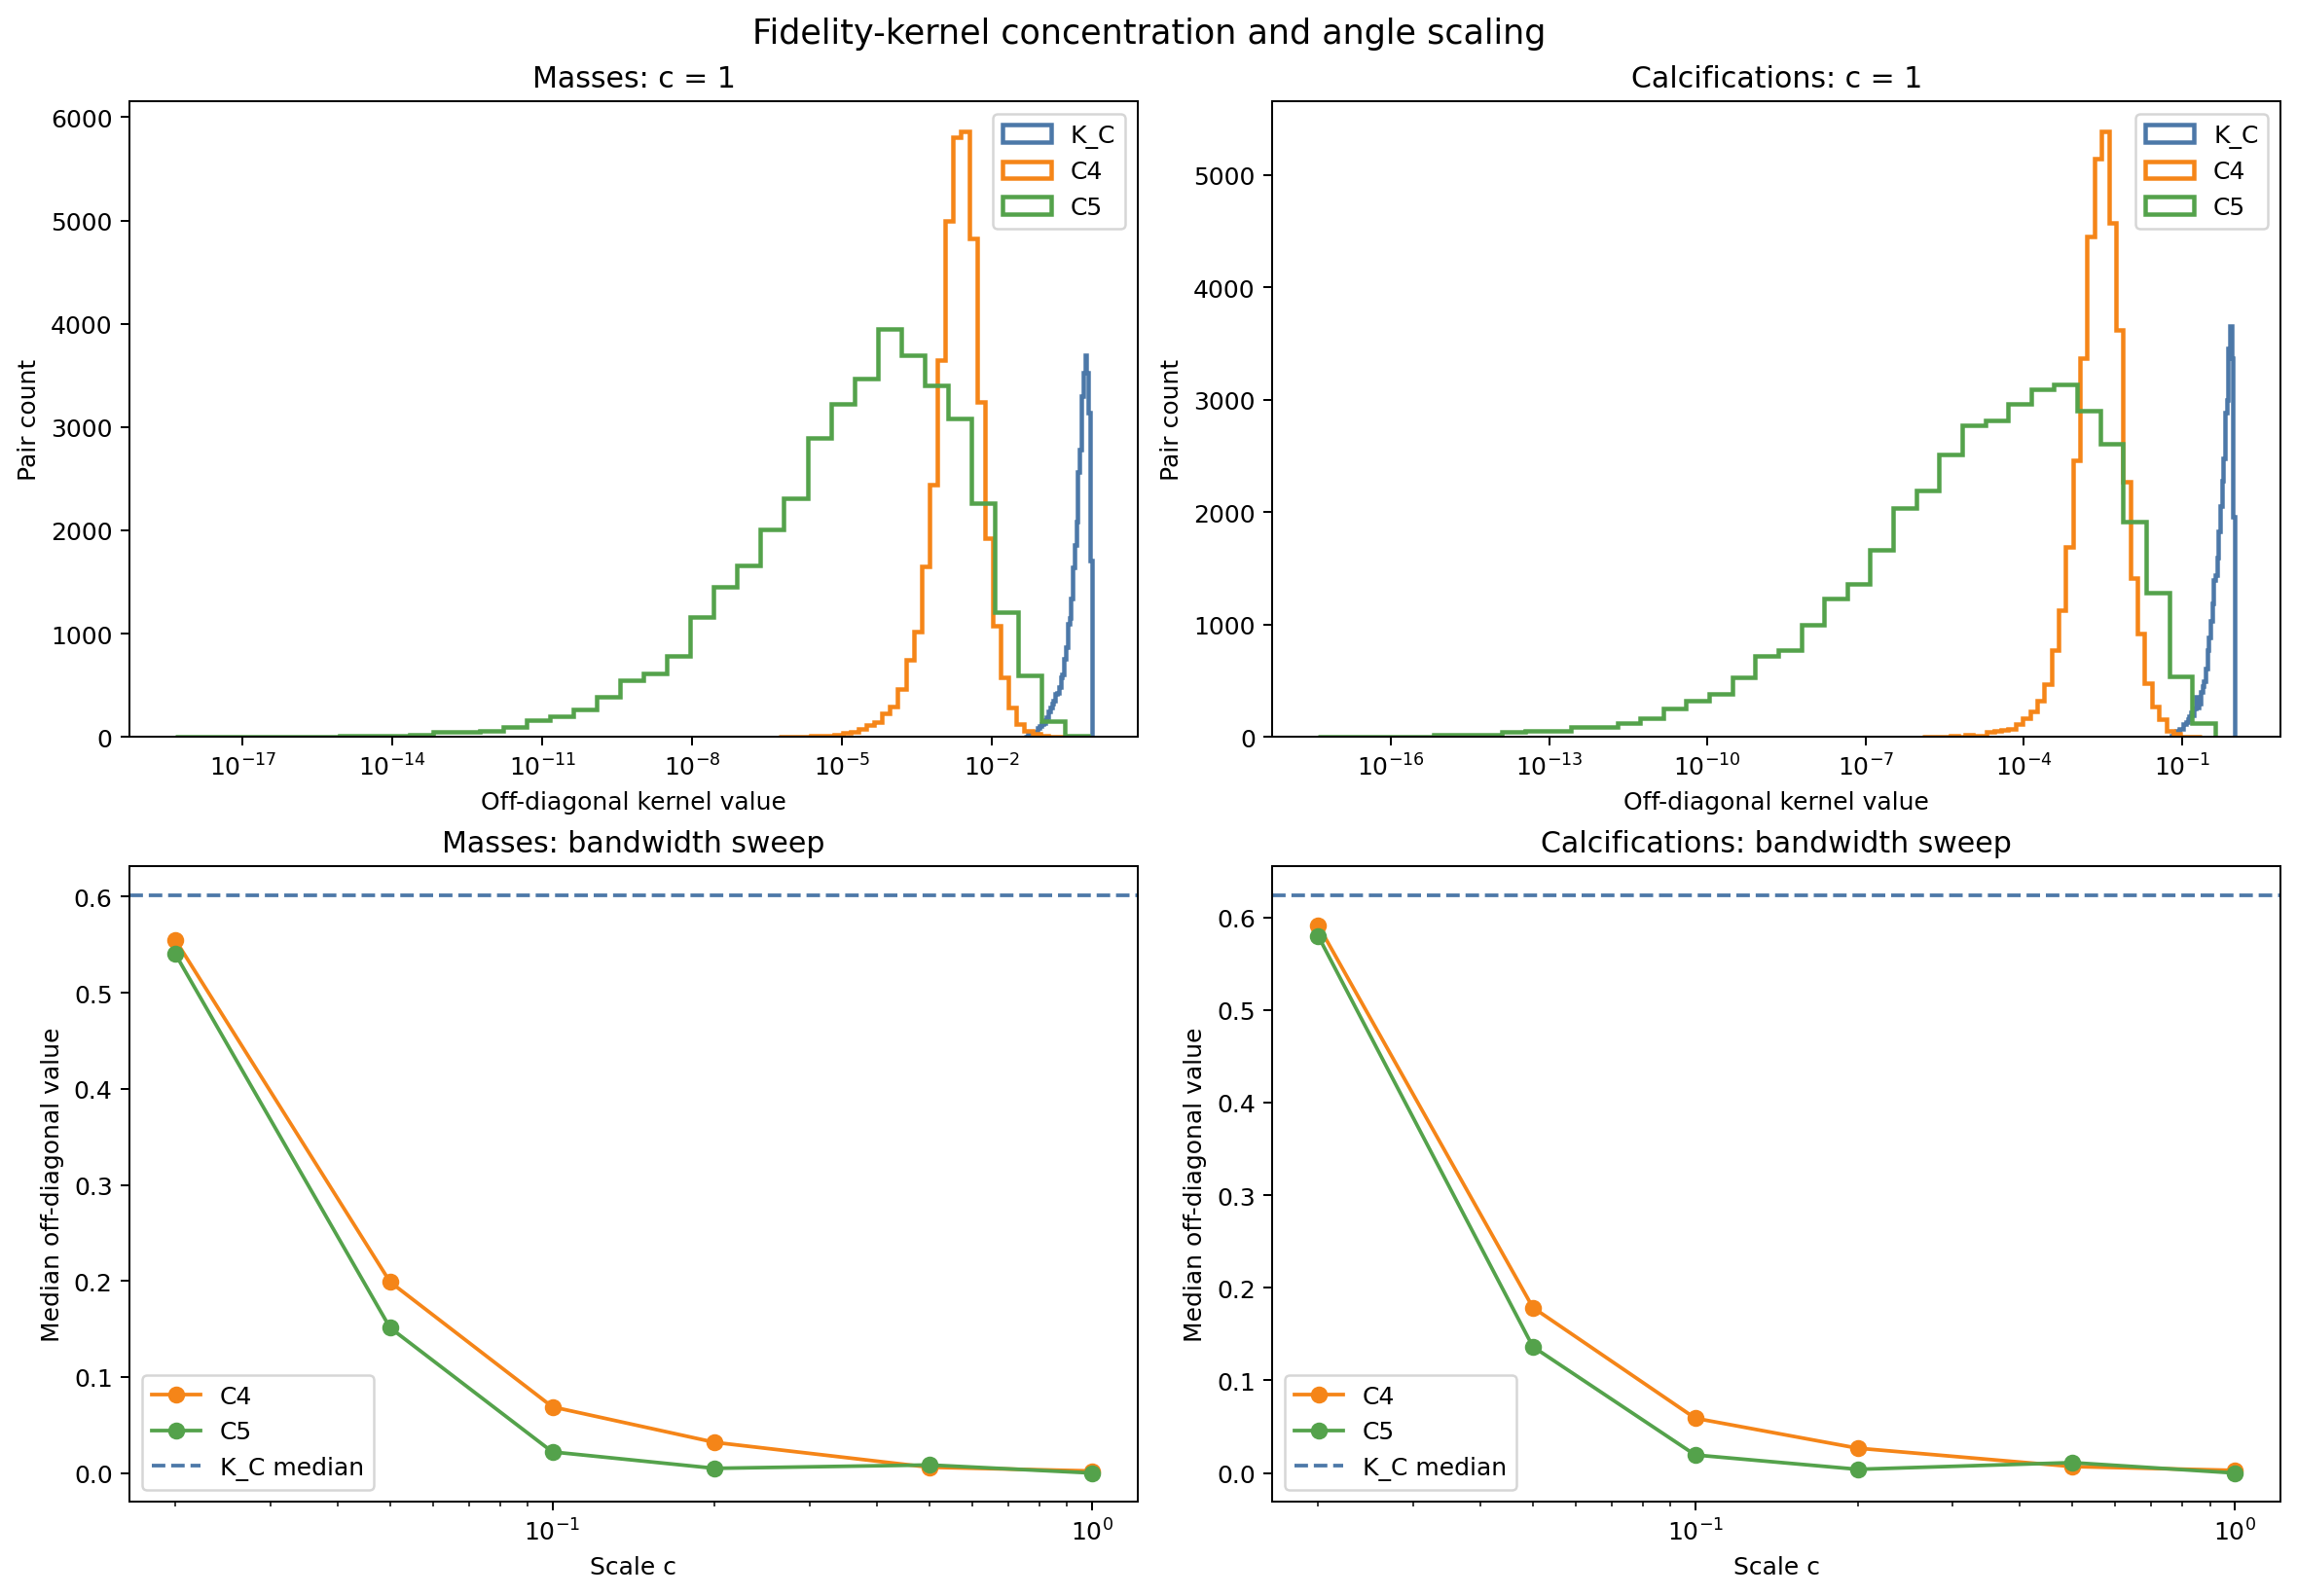
\includegraphics[width=\columnwidth]{M5_kernel_concentration.png}
% fuente: Docs/capitulos/6_Resultados/6.2_separabilidad.tex:12, Docs/capitulos/6_Resultados/6.2_separabilidad.tex:45, Docs/capitulos/6_Resultados/6.2_separabilidad.tex:185 (H-031, H-037; 5b_concentracion_kernel.csv)
\caption{Distribución de los valores fuera de la diagonal en las matrices de kernel cuántico (C4 y C5) frente al kernel clásico RBF a $c = 1$ (arriba) y mediana fuera de la diagonal en función del factor de escala angular $c$ (abajo).}
\label{fig:kernel_conc}
\end{figure}

% fuente: Docs/capitulos/6_Resultados/6.2_separabilidad.tex:58, Docs/capitulos/6_Resultados/6.2_separabilidad.tex:68, Docs/capitulos/6_Resultados/6.2_separabilidad.tex:76 (H-038, H-039; 6_alineamiento_kernel.csv, 6_dimension_efectiva.csv, 6_diferencia_geometrica_resumen.csv)
En las métricas formales sobre kernels a $c = 1$, ninguna transformación cuántica superó al kernel RBF. El exceso de KTA centrado sobre 1\,000 permutaciones fue en masas de 0.049 ($p < 0.001$) para el RBF, frente a 0.003 ($p = 0.002$) en C4 y 0.005 ($p = 0.003$) en C5; en calcificaciones fue de 0.151 ($p < 0.001$) para el RBF, frente a 0.006 ($p < 0.001$) en C4 y 0.007 ($p = 0.003$) en C5, lo que representa apenas entre el 4\,\% y el 10\,\% del exceso clásico (estando los valores brutos de KTA centrada de C4 y C5, de 0.073 a 0.077, dominados por la cota $1/\sqrt{N-1} \approx 0.071$). La dimensión efectiva normalizada ($d_{\mathrm{eff}}$ sobre 200) alcanzó 184.0 (C4) y 171.3 (C5) en masas, y 187.7 (C4) y 167.6 (C5) en calcificaciones, frente a 2.8 y 2.6 en el RBF, saturando casi todo el espacio muestral. La diferencia geométrica regularizada mínima frente a la batería de kernels clásicos fue $g = 1.433$ (C4) y $1.511$ (C5) en masas, y $g = 1.400$ (C4) y $1.701$ (C5) en calcificaciones (descendiendo a un rango de 1.31 a 1.70 al ampliar la batería gaussiana), cumpliéndose $g \ll \sqrt{N} \approx 14.1$ \cite{huang2021power}; sin regularizar, $g$ toma valores de 306 a 388 por el condicionamiento numérico de $K_C^{-1}$ (cota teórica cercana a 410 para $K_Q = I$).

% fuente: Docs/capitulos/6_Resultados/6.2_separabilidad.tex:110, Docs/capitulos/6_Resultados/6.2_separabilidad.tex:139, Docs/capitulos/6_Resultados/6.2_separabilidad.tex:166, Docs/capitulos/6_Resultados/6.2_separabilidad.tex:184, Docs/capitulos/6_Resultados/6.2_separabilidad.tex:197 (H-031, H-036, H-037, H-039, H-040, H-041, H-055, D-029; 5b_concentracion_kernel.csv, 6_metricas_embedding.csv, X2_auc_pares.csv, X3_comparacion_k8_k12.csv, X9_resumen_familia_a.csv)
Sobre los vectores de representación $\langle Z_i \rangle$, las condiciones clásicas C1 a C3 aventajaron igualmente a C4 y C5 en ambos subconjuntos: en masas, el índice de Davies-Bouldin fue de 4.301 en C1 y C2 frente a 5.898 en C4 y 13.346 en C5, la razón de Fisher $J$ fue de 0.669 en C1 y C2 (0.781 en C3) frente a 0.449 en C4 y 0.668 en C5, y el KTA lineal fue de 0.070 en C1 y C2 frente a 0.041 en C4 y 0.012 en C5; en calcificaciones, Davies-Bouldin fue de 2.387 en C1 y C2 frente a 6.890 en C4 y 6.247 en C5, Fisher $J$ fue de 1.284 en C1 y C2 (1.390 en C3) frente a 0.399 en C4 y 0.753 en C5, y el KTA lineal fue de 0.181 en C1 y C2 frente a 0.031 en C4 y 0.041 en C5 (con C1 y C2 coincidiendo dentro de $< 10^{-14}$). Esta conclusión se mantuvo invariante en 20 submuestras de 200 lesiones y sobre la totalidad del entrenamiento en el experimento X9 (donde el exceso de KTA fue de 0.055 en el RBF frente a 0.006 y 0.009 en las 1\,318 masas, y de 0.148 frente a 0.018 y 0.020 en las 1\,546 calcificaciones, con $g$ entre 2.95 y 3.25 frente a $\sqrt{N}$ de 36.3 y 39.3), así como en el AUC de pares de X2 (0.523 y 0.575 en el RBF frente a 0.508 a 0.510 y 0.520 a 0.547 en C4/C5). Al contraer los ángulos hacia $c = 0.02$, la mediana fuera de la diagonal subió de 0.54 a 0.59 y el exceso de KTA a 0.043 y 0.143, pero el kernel cuántico presentó una correlación de 0.99997 en masas y 0.99999 en calcificaciones con un circuito que omite el producto cruzado $x_i x_j$, indicando que la concentración solo desaparece cuando se desactiva la interacción de segundo orden. De forma análoga, al reducir el registro a $k = 8$ qubits (X3), el exceso de KTA cuántico aumentó entre 1.7 y 4.6 veces (0.011 a 0.024) y $g$ subió a un rango de 1.71 a 3.23, permaneciendo por debajo del RBF y de $\sqrt{N} = 14.1$.

\subsection{Clasificación supervisada y origen de la pérdida (M7, X4--X8)}

% fuente: Docs/capitulos/6_Resultados/6.3_clasificacion.tex:10, Docs/capitulos/6_Resultados/6.3_clasificacion.tex:13, Docs/capitulos/6_Resultados/6.3_clasificacion.tex:16, Docs/capitulos/6_Resultados/6.3_clasificacion.tex:19, Docs/capitulos/6_Resultados/6.3_clasificacion.tex:21, Docs/capitulos/6_Resultados/6.3_clasificacion.tex:40, Docs/capitulos/6_Resultados/6.3_clasificacion.tex:43 (H-042, H-043; 7_test.csv, 7_cv_resumen.csv, 7_test_diferencias.csv)
La Tabla~\ref{tab:m7_compacta} y la Fig.~\ref{fig:m7_roc} resumen el desempeño del perceptrón multicapa sobre las cinco condiciones. El control nulo C2 no difirió significativamente de C1 en el conjunto de prueba (diferencias pareadas C2 $-$ C1 de $-0.011$ [$-0.061$, $0.038$], $p = 0.659$ en masas y $+0.020$ [$-0.026$, $0.067$], $p = 0.377$ en calcificaciones). Por el contrario, las condiciones cuánticas registraron caídas estadísticamente significativas frente a C1: en masas, C4 $-$ C1 fue de $-0.122$ [$-0.202$, $-0.044$] ($p = 0.003$) y C5 $-$ C1 de $-0.070$ [$-0.140$, $-0.004$] ($p = 0.044$); en calcificaciones, C4 $-$ C1 fue de $-0.135$ [$-0.208$, $-0.061$] ($p = 0.001$) y C5 $-$ C1 de $-0.118$ [$-0.182$, $-0.046$] ($p < 0.001$), manteniendo las cuatro diferencias su significancia bajo la corrección escalonada de Holm a nivel $\alpha = 0.05$. La diferencia entre C5 y C4 no fue significativa en ningún subconjunto ($0.051$ en masas y $0.017$ en calcificaciones). La brecha persistió ante variaciones de semilla del MLP (dispersión máxima de 0.039 en validación cruzada), arquitecturas alternas (16-8 y 64-32), entrenamiento forzado a 200 épocas sin parada temprana (donde C4 y C5 descendieron a 0.533 y 0.557 en masas y a 0.596 y 0.631 en calcificaciones), aumento a dos repeticiones en el circuito variacional (con el que C5 pasó a 0.603 y 0.682 manteniendo diferencias negativas frente a C1 de $-0.048$ y $-0.086$) y reducción a $k = 8$ qubits.

% fuente: Docs/capitulos/6_Resultados/6.3_clasificacion.tex:10, Docs/capitulos/6_Resultados/6.3_clasificacion.tex:13, Docs/capitulos/6_Resultados/6.3_clasificacion.tex:21 (H-042; 7_test.csv, 7_cv_resumen.csv, Docs/tablas/m7_clasificacion.tex)
\begin{table}[t]
\centering
\caption{Clasificación con el mismo MLP sobre las cinco representaciones (M7, $k = 12$; valores de \texttt{m7\_clasificacion.tex}).}
\label{tab:m7_compacta}
\setlength{\tabcolsep}{3.2pt}
\footnotesize
\begin{tabular}{l c c r r}
\toprule
Condición & AUC en VC & AUC en prueba [IC 95\,\%] & F1 & Exact. \\
\midrule
\multicolumn{5}{l}{\textit{Masas}} \\
\quad C1 & 0.652 $\pm$ 0.068 & 0.651 [0.578, 0.724] & 0.519 & 0.638 \\
\quad C2 & 0.641 $\pm$ 0.059 & 0.641 [0.572, 0.710] & 0.512 & 0.616 \\
\quad C3 & 0.648 $\pm$ 0.055 & 0.646 [0.572, 0.721] & 0.502 & 0.606 \\
\quad C4 & 0.565 $\pm$ 0.079 & 0.530 [0.473, 0.587] & 0.386 & 0.529 \\
\quad C5 & 0.563 $\pm$ 0.024 & 0.581 [0.521, 0.644] & 0.456 & 0.571 \\
\multicolumn{5}{l}{\textit{Calcificaciones}} \\
\quad C1 & 0.742 $\pm$ 0.038 & 0.769 [0.694, 0.836] & 0.665 & 0.666 \\
\quad C2 & 0.758 $\pm$ 0.046 & 0.788 [0.719, 0.851] & 0.669 & 0.693 \\
\quad C3 & 0.739 $\pm$ 0.036 & 0.758 [0.685, 0.826] & 0.652 & 0.653 \\
\quad C4 & 0.640 $\pm$ 0.041 & 0.633 [0.558, 0.700] & 0.504 & 0.607 \\
\quad C5 & 0.667 $\pm$ 0.035 & 0.652 [0.571, 0.725] & 0.565 & 0.571 \\
\bottomrule
\end{tabular}
\par\smallskip
\parbox{\columnwidth}{\scriptsize VC: media $\pm$ desviación estándar en 5 pliegues agrupados por paciente. Prueba: conjunto oficial evaluado una vez por modelo; IC por \textit{bootstrap} por paciente con 2\,000 réplicas. Umbral de 0.5 para F1 y exactitud.}
\end{table}

\begin{figure}[t]
\centering
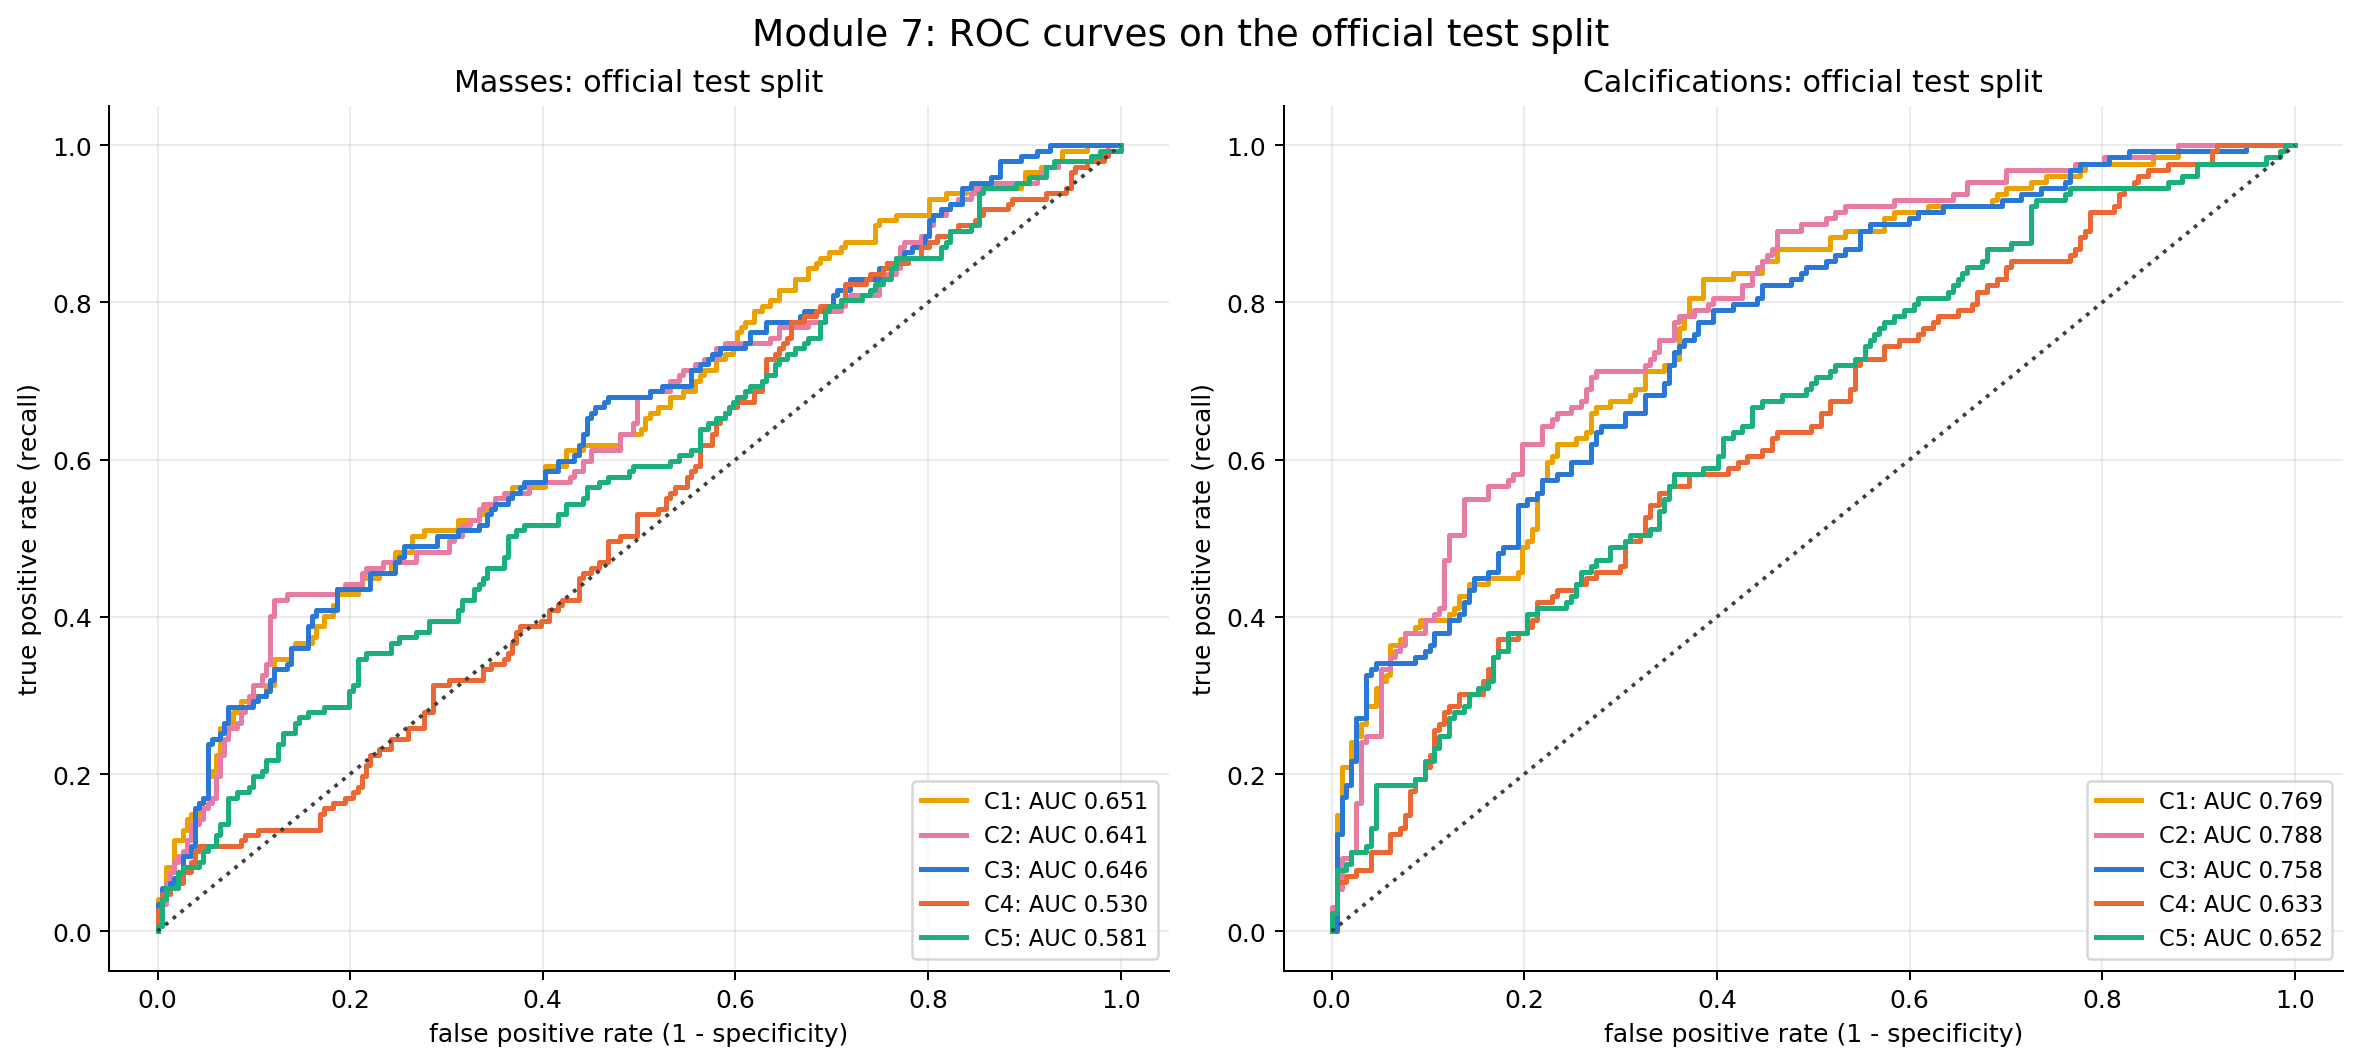
\includegraphics[width=\columnwidth]{M7_roc_test.png}
% fuente: Docs/capitulos/6_Resultados/6.3_clasificacion.tex:10, Docs/capitulos/6_Resultados/6.3_clasificacion.tex:13, Docs/capitulos/6_Resultados/6.3_clasificacion.tex:34 (H-042; 7_test.csv)
\caption{Curvas ROC sobre el conjunto de prueba oficial para masas y calcificaciones bajo las cinco condiciones de representación.}
\label{fig:m7_roc}
\end{figure}

% fuente: Docs/capitulos/6_Resultados/6.3_clasificacion.tex:56, Docs/capitulos/6_Resultados/6.3_clasificacion.tex:69, Docs/capitulos/6_Resultados/6.4_qsvm_ventaja.tex:10, Docs/capitulos/6_Resultados/6.4_qsvm_ventaja.tex:13, Docs/capitulos/6_Resultados/6.4_qsvm_ventaja.tex:23, Docs/capitulos/6_Resultados/6.4_qsvm_ventaja.tex:33, Docs/capitulos/6_Resultados/6.4_qsvm_ventaja.tex:36, Docs/capitulos/6_Resultados/6.4_qsvm_ventaja.tex:41, Docs/capitulos/6_Resultados/6.4_qsvm_ventaja.tex:54 (H-044, H-045, H-046, H-047, H-048, H-053, H-054; X4_test.csv, X4_test_diferencias.csv, X5_auditoria.csv, X6_test.csv, X6_etiquetas_construidas.csv, X7_resumen.csv, X8_test.csv)
Los experimentos X4 a X8 permitieron identificar las causas de este comportamiento. En X4, una máquina de vectores de soporte sobre el kernel cuántico completo de C4 (QSVM) alcanzó en el conjunto de prueba un AUC de 0.628 [0.55, 0.70] en masas y 0.759 [0.69, 0.83] en calcificaciones, resultado estadísticamente indistinguible del SVM RBF clásico (0.649 y 0.769; diferencias de $-0.02$ y $-0.01$) y superior en $+0.10$ [$0.03$, $0.17$] y $+0.13$ [$0.05$, $0.20$] al MLP entrenado sobre las expectativas $\langle Z_i \rangle$ de C4. Esto indica que el estado cuántico de $2^{12} = 4\,096$ amplitudes conserva información diagnóstica comparable a la clásica y que la caída del Módulo~7 ocurre al proyectarlo sobre 12 observables locales $\langle Z_i \rangle$. Dicha pérdida no obedece al sorteo único de $\boldsymbol{\theta}$ (en X7, diez sorteos independientes con semillas 42 a 51 produjeron variaciones de 0.040 a 0.110 de AUC pero dejaron las 40 evaluaciones entre 0.03 y 0.18 por debajo de C1) ni a la ausencia de entrenamiento variacional (en X8, optimizar $\boldsymbol{\theta}$ junto con el MLP aportó variaciones no significativas de $+0.003$ a $+0.041$ en prueba, manteniéndose entre $-0.066$ y $-0.118$ por debajo de C1). La auditoría independiente X5 superó las 25 pruebas de verificación y reprodujo bit a bit los 81 archivos de resultados y los 10\,704 archivos preprocesados. Finalmente, en la búsqueda anidada simétrica X6 (28 candidatos cuánticos frente a 12 clásicos), el mejor modelo cuántico no superó al clásico en prueba ($0.656$ frente a $0.652$ en masas; $0.755$ frente a $0.760$ en calcificaciones) y convergió a escalas reducidas ($c = 0.05$ y $0.2$) que emulan un kernel gaussiano, mientras que los kernels proyectados elevaron $g$ a un rango de 6 a 9 pero redujeron el AUC en $-0.11$ y $-0.06$ sobre las etiquetas reales; en cambio, al aplicar el etiquetado diseñado según Huang et al.~\cite{huang2021power}, el kernel proyectado cuántico alcanzó un AUC de 0.998 en masas y 0.994 en calcificaciones frente a 0.800 y 0.824 del mejor clásico, confirmando que el protocolo detecta ventaja cuando el etiquetado se alinea con la geometría del circuito.

\subsection{Evaluación comparativa y restricciones del simulador (M8, OE-6)}

% fuente: Docs/capitulos/6_Resultados/6.5_comparacion.tex:13, Docs/capitulos/6_Resultados/6.5_comparacion.tex:16, Docs/capitulos/6_Resultados/6.5_comparacion.tex:33, Docs/capitulos/6_Resultados/6.5_comparacion.tex:36 (H-049, H-050; 8_spearman.csv, 8_masas_vs_calcificaciones.csv, 8_descriptores_radiologo.csv)
En el Módulo~8, los 48 coeficientes descriptivos de correlación de rangos de Spearman $\rho_s$ entre las métricas de separabilidad y el AUC-ROC resultaron positivos (en el rango de 0.67 a 0.97; en la muestra primaria a $k = 12$, entre 0.718 y 0.821 en masas y entre 0.667 y 0.975 en calcificaciones, donde 0.975 es el máximo teórico con el empate exacto C1 = C2 y $p = 4/120 \approx 0.033$), situando de forma consistente a C1--C3 por delante de C4--C5. Respecto a la asimetría entre subproblemas, una regresión logística sobre los descriptores anotados por el radiólogo mostró mayor separabilidad en masas que en calcificaciones (AUC de 0.872 frente a 0.825), pero con las 67 características radiómicas el orden se invirtió (0.693 en masas frente a 0.800 en calcificaciones; 0.668 frente a 0.745 con 12 variables), mostrando que las características radiómicas estándar capturan mejor la morfología de las calcificaciones que los márgenes espiculados de las masas, mientras que la penalización cuántica C4 $-$ C1 fue similar en ambos subconjuntos ($-0.12$ y $-0.14$).

% fuente: Docs/capitulos/6_Resultados/6.3_clasificacion.tex:72, Docs/capitulos/6_Resultados/6.6_restricciones_simulador.tex:10, Docs/capitulos/6_Resultados/6.6_restricciones_simulador.tex:13, Docs/capitulos/6_Resultados/6.6_restricciones_simulador.tex:23, Docs/capitulos/6_Resultados/6.6_restricciones_simulador.tex:26, Docs/capitulos/6_Resultados/6.7_lecciones_implementacion.tex:65 (H-019, H-032, H-051, H-052, H-054; 8_oe6_qubits.csv, 8_oe6_shots_embedding.csv, 8_oe6_shots_kernel.csv, 8_oe6_resumen.csv, X8_costo_gradiente.csv)
En el análisis de viabilidad operacional (OE-6) sobre un procesador Apple M3 con 16\,GiB de RAM, el tiempo de simulación por vector de estado escaló como $2^k$ (multiplicándose por $\approx 1.9$ por qubit a partir de $k = 20$, hasta unos 75\,s por estado a $k = 28$). Bajo un límite de 24 horas y 8\,GiB de memoria, almacenar un vector de estado es viable hasta $k = 29$ qubits, precomputar los \textit{embeddings} de todo el conjunto admite 25 a 26 qubits y calcular el kernel de $200 \times 200$ por \textit{compute-uncompute} soporta 22 a 23 qubits; en cambio, entrenar $\boldsymbol{\theta}$ durante 50 épocas mediante \textit{parameter-shift} cuesta 5.16\,s por lesión a $k = 12$ con \texttt{EstimatorQNN} (48 ejecuciones, unas 205~h por mapa), e incluso con el tiempo mínimo de simulación por circuito, una cota inferior, deja de caber en un día a partir de 14 a 15 qubits. Tanto la evaluación del kernel mediante productos internos de vectores de estado (\texttt{Fidelity\allowbreak Statevector\allowbreak Kernel}, que reduce el cálculo de 41 minutos a 1.5\,s) como la retropropagación analítica (1.4\,ms por lesión, unas 3\,600 veces más rápida que \textit{parameter-shift} con discrepancia de $1.8 \times 10^{-15}$) son atajos exclusivos de la simulación clásica, irrealizables en hardware físico por el colapso del estado al medir; asimismo, se documentó que \texttt{EstimatorQNN} fija por omisión una precisión de 0.015625 que inyecta ruido gaussiano si no se declara precisión cero explícita. Al simular mediciones discretas con 1\,024 disparos, el ruido representa el 55\,\% y el 65\,\% de la dispersión entre lesiones en C4 y el 17\,\% en C5, pero el MLP conserva el AUC en validación cruzada a menos de 0.02 del valor exacto (0.548 frente a 0.565 y 0.630 frente a 0.640 en C4; 0.565 frente a 0.563 y 0.654 frente a 0.667 en C5). No obstante, para el kernel cuántico a $c = 1$ con 1\,024 disparos, el 21.5\,\% de los pares en masas y el 15.7\,\% en calcificaciones leerían exactamente cero en C4, y el 74.5\,\% y el 71.6\,\% en C5; acotar el error relativo al 10\,\% exigiría una mediana de 46\,000 y 35\,000 disparos por par en C4 y de 3.1 y 3.2 millones en C5.

\section{Conclusiones}

% fuente: Docs/capitulos/6_Resultados/6.2_separabilidad.tex:12, Docs/capitulos/6_Resultados/6.2_separabilidad.tex:59, Docs/capitulos/6_Resultados/6.2_separabilidad.tex:77, Docs/capitulos/6_Resultados/6.3_clasificacion.tex:10, Docs/capitulos/6_Resultados/6.3_clasificacion.tex:13, Docs/capitulos/6_Resultados/6.4_qsvm_ventaja.tex:13, Docs/capitulos/6_Resultados/6.4_qsvm_ventaja.tex:54, Docs/capitulos/6_Resultados/6.6_restricciones_simulador.tex:13, Docs/capitulos/6_Resultados/6.6_restricciones_simulador.tex:26, Docs/capitulos/6_Resultados/6.8_sintesis.tex:35 (H-031, H-039, H-042, H-044, H-048, H-051, H-052)
Los resultados experimentales responden de manera negativa y verificable a la pregunta de investigación: bajo el diseño predefinido ($k = 12$, una repetición y escala $c = 1$), las transformaciones cuánticas implementadas con \texttt{zz\_\allowbreak feature\_\allowbreak map} y \texttt{pauli\_\allowbreak feature\_\allowbreak map} $(Y, ZZ)$ no incrementaron la separabilidad de clases benigno/maligno de las características radiómicas del CBIS-DDSM, sino que la redujeron respecto a las representaciones clásicas, y dicha pérdida se trasladó en la misma dirección al clasificador neuronal (con caídas de 0.07 a 0.14 de AUC-ROC en el conjunto de prueba). El análisis identifica tres mecanismos causales: (1) la codificación en un espacio de Hilbert de $2^{12}$ dimensiones sitúa a las lesiones casi ortogonales entre sí (fidelidad mediana de 0.0022 a 0.0029 en C4 y de 0.000031 a 0.000032 en C5, con $g$ de 1.400 a 1.701 frente a $\sqrt{N} \approx 14.1$), y contraer los ángulos solo alivia la concentración cuando desactiva el término de interacción $x_i x_j$; (2) la caída clasificatoria del Módulo~7 se origina en la lectura de 12 valores esperados $\langle Z_i \rangle$, dado que una QSVM sobre el kernel cuántico de C4 recupera entre $+0.10$ y $+0.13$ de AUC-ROC e iguala al SVM clásico; y (3) las etiquetas clínicas reales no se alinean con la geometría inducida por las familias de circuitos evaluadas, a diferencia del control con etiquetado diseñado según Huang et al.~\cite{huang2021power}, donde el kernel proyectado alcanza un AUC de 0.998 y 0.994. En términos de viabilidad práctica en salud (OE-6), las limitantes primordiales antes que el número de qubits son el coste de estimar gradientes físicos por \textit{parameter-shift} (unas 205~h por mapa a $k = 12$) y la concentración exponencial del kernel, que haría que entre el 15.7\,\% y el 74.5\,\% de las entradas resultaran nulas a 1\,024 disparos. Estas conclusiones se acotan al uso de un único conjunto de mamografías digitalizadas sin calibración física, a la reducción a 12 características univariantes y a simulación ideal sin ruido de dispositivo, dejando como trabajo futuro la exploración de codificaciones diseñadas específicamente a partir de invarianzas morfológicas del dominio mamográfico.

\begin{thebibliography}{99}

\bibitem{Bray2024GLOBOCAN}
F. Bray, M. Laversanne, H. Sung, J. Ferlay, R. L. Siegel, I. Soerjomataram y A. Jemal, ``Global cancer statistics 2022: GLOBOCAN estimates of incidence and mortality worldwide for 36 cancers in 185 countries,'' \textit{CA: A Cancer Journal for Clinicians}, vol. 74, no. 3, pp. 229--263, 2024, doi: \url{https://doi.org/10.3322/caac.21834}.

\bibitem{INEGI2025}
Instituto Nacional de Estadística y Geografía, ``Estadísticas de cáncer de mama,'' 2025. [En línea]. Disponible en: \url{https://www.inegi.org.mx/contenidos/saladeprensa/aproposito/2025/EAP_CancerMama_25.pdf}

\bibitem{Wang2020DeepLearning}
X. Wang, G. Liang, Y. Zhang, H. Blanton, Z. Bessinger y N. Jacobs, ``Inconsistent performance of deep learning models on mammogram classification,'' \textit{Journal of the American College of Radiology}, vol. 17, no. 6, pp. 796--803, 2020, doi: \url{https://doi.org/10.1016/j.jacr.2020.01.006}.

\bibitem{havlicek2019supervised}
V. Havl{\'{i}}{\v{c}}ek, A. D. C{\'{o}}rcoles, K. Temme, A. W. Harrow, A. Kandala, J. M. Chow y J. M. Gambetta, ``Supervised learning with quantum-enhanced feature spaces,'' \textit{Nature}, vol. 567, pp. 209--212, 2019, doi: \url{https://doi.org/10.1038/s41586-019-0980-2}.

\bibitem{schuld2019quantum}
M. Schuld y N. Killoran, ``Quantum machine learning in feature {H}ilbert spaces,'' \textit{Physical Review Letters}, vol. 122, no. 4, p. 040504, 2019, doi: \url{https://doi.org/10.1103/PhysRevLett.122.040504}.

\bibitem{Mari2020Transfer}
A. Mari, T. R. Bromley, J. Izaac, M. Schuld y N. Killoran, ``Transfer learning in hybrid classical-quantum neural networks,'' \textit{Quantum}, vol. 4, p. 340, 2020, doi: \url{https://doi.org/10.22331/q-2020-10-09-340}.

\bibitem{Bowles2024Benchmarking}
J. Bowles, S. Ahmed y M. Schuld, ``Better than classical? The subtle art of benchmarking quantum machine learning models,'' \textit{arXiv preprint} arXiv:2403.07059, 2024, doi: \url{https://doi.org/10.48550/arXiv.2403.07059}.

\bibitem{huang2021power}
H.-Y. Huang, M. Broughton, M. Mohseni, R. Babbush, S. Boixo, H. Neven y J. R. McClean, ``Power of data in quantum machine learning,'' \textit{Nature Communications}, vol. 12, p. 2631, 2021, doi: \url{https://doi.org/10.1038/s41467-021-22539-9}.

\bibitem{Thanasilp2024}
S. Thanasilp, S. Wang, M. Cerezo y Z. Holmes, ``Exponential concentration in quantum kernel methods,'' \textit{Nature Communications}, vol. 15, no. 1, p. 5200, 2024, doi: \url{https://doi.org/10.1038/s41467-024-49287-w}.

\bibitem{Azevedo2022QuantumTransfer}
V. Azevedo, C. Silva y I. Dutra, ``Quantum transfer learning for breast cancer detection,'' \textit{Quantum Machine Intelligence}, vol. 4, no. 1, p. 5, 2022, doi: \url{https://doi.org/10.1007/s42484-022-00062-4}.

\bibitem{Lee2017CBISDDSM}
R. S. Lee, F. Gimenez, A. Hoogi, K. K. Miyake, M. Gorovoy y D. L. Rubin, ``A curated mammography data set for use in computer-aided detection and diagnosis research,'' \textit{Scientific Data}, vol. 4, no. 1, p. 170177, 2017, doi: \url{https://doi.org/10.1038/sdata.2017.177}.

\bibitem{Zwanenburg2020IBSI}
A. Zwanenburg, M. Valli\`eres, M. A. Abdalah \textit{et al.}, ``The Image Biomarker Standardization Initiative: Standardized quantitative radiomics for high-throughput image-based phenotyping,'' \textit{Radiology}, vol. 295, no. 2, pp. 328--338, 2020, doi: \url{https://doi.org/10.1148/radiol.2020191145}.

\bibitem{vanGriethuysen2017}
J. J. M. van Griethuysen \textit{et al.}, ``Computational radiomics system to decode the radiographic phenotype,'' \textit{Cancer Research}, vol. 77, no. 21, pp. e104--e107, 2017, doi: \url{https://doi.org/10.1158/0008-5472.CAN-17-0339}.

\bibitem{Guyon2003}
I. Guyon y A. Elisseeff, ``An introduction to variable and feature selection,'' \textit{Journal of Machine Learning Research}, vol. 3, pp. 1157--1182, 2003. [En línea]. Disponible en: \url{https://jmlr.org/papers/v3/guyon03a.html}

\bibitem{Cortes2012}
C. Cortes, M. Mohri y A. Rostamizadeh, ``Algorithms for learning kernels based on centered alignment,'' \textit{Journal of Machine Learning Research}, vol. 13, no. 28, pp. 795--828, 2012. [En línea]. Disponible en: \url{https://jmlr.org/papers/v13/cortes12a.html}

\bibitem{davies1979cluster}
D. L. Davies y D. W. Bouldin, ``A cluster separation measure,'' \textit{IEEE Transactions on Pattern Analysis and Machine Intelligence}, vol. 1, no. 2, pp. 224--227, 1979, doi: \url{https://doi.org/10.1109/TPAMI.1979.4766909}.

\bibitem{fisher1936use}
R. A. Fisher, ``The use of multiple measurements in taxonomic problems,'' \textit{Annals of Eugenics}, vol. 7, no. 2, pp. 179--188, 1936, doi: \url{https://doi.org/10.1111/j.1469-1809.1936.tb02137.x}.

\end{thebibliography}

\end{document}
